\def\year{2017}\relax
%File: formatting-instruction.tex
\documentclass[letterpaper]{article}
\usepackage{aaai17}
\usepackage{times}
\usepackage{helvet}
\usepackage{courier}
\usepackage{url} 
\usepackage{multicol}
\usepackage{array}
\usepackage{xcolor}

\usepackage{graphicx}
\graphicspath{ {images/} }

\usepackage[breaklinks=true]{hyperref}
\usepackage{breakcites}
\frenchspacing
\setlength{\pdfpagewidth}{8.5in}
\setlength{\pdfpageheight}{11in}
\pdfinfo{
/Title (Nasty, Brutish, and Short: 
What Makes Election News Popular on Twitter?)
/Author (Anonymous)}
\setcounter{secnumdepth}{0}  
 \begin{document}
% The file aaai.sty is the style file for AAAI Press 
% proceedings, working notes, and technical reports.
%
\title{Nasty, Brutish, and Short:\\
What Makes Election News Popular on Twitter?}
\author{Anonymous\\
%Association for the Advancement of Artificial Intelligence\\
%2275 East Bayshore Road, Suite 160\\
%Palo Alto, California 94303\\
}
\maketitle
\begin{abstract}
Lorem ipsum dolor. Sit amet mauris. Sed ut eu aliquam integer nibh vitae adipiscing diam mauris erat est. Libero amet parturient. Nulla vehicula dui elit cras ante. Lacus imperdiet scelerisque felis bibendum dolorem maecenas amet quis. Magna ultricies faucibus esse convallis quis. Leo pretium habitasse. Nam cursus aptent bibendum nulla per conubia tellus tincidunt. Eget tellus sed ut vel erat.
Lorem ipsum dolor. Sit amet mauris. Sed ut eu aliquam integer nibh vitae adipiscing diam mauris erat est. Libero amet parturient. Nulla vehicula dui elit cras ante. Lacus imperdiet scelerisque felis bibendum dolorem maecenas amet quis. Magna ultricies faucibus esse convallis quis. Leo pretium habitasse. Nam cursus aptent bibendum nulla per conubia tellus tincidunt. Eget tellus sed ut vel erat.
Lorem ipsum dolor. Sit amet mauris. Sed ut eu aliquam integer nibh vitae adipiscing diam mauris erat est. Libero amet parturient. Nulla vehicula dui elit cras ante. Lacus imperdiet scelerisque felis bibendum dolorem maecenas amet quis. Magna ultricies faucibus esse convallis quis. Leo pretium habitasse. Nam cursus aptent bibendum nulla per conubia tellus tincidunt. Eget tellus sed ut vel erat.


\end{abstract}

 
\section{Introduction}
In the changing landscape of both journalism and politics, social media is playing an increasingly large role in mobilizing and spreading information to citizens. A Pew Research survey from August 2015 showed that nearly two-thirds of adults in the U.S. who are on Twitter use the platform to get news \cite{pew-Twitter-news}. 

In 2008, President Barack Obama's winning campaign was largely attributed to the success of his social media strategy, the first example of its kind. By establishing an online presence that recruited more than 3 million individual contributors and 5 million volunteers, Obama was able to create a grassroots political movement \cite{cogburn2011networked}. Publicity and public sound bites matter-- especially when it’s free and has the potential to go viral.

Although social media messages are less able to be carefully controlled in comparison to paid advertisements, they also have the potential to reach a wider audience. Reactions to an article shared by one potential voter now have the ability to be broadcast and spread to millions of others in a real-time, public sphere. 

%Measuring the way that stories grow and spread has become an important part of the equation to understanding public discourse.

%\subsection{From Reader to Relayer}
The popularity of sharing articles on social media also marks an important shift in the role of the news consumer from armchair reader to information propagator. Whereas news used to be broadcast to the reader, now each reader has the potential to broadcast stories to his or her own audience. Sharing a story requires a level of interest and activation on the part of the reader beyond simply reading a story; yet often, this trigger is predictably emotional in nature. 

In a 2011 study of the New York Time’s ``most emailed list'', Berger and Milkman found that the potential for a news story to go viral is partially driven by physiological arousal, defined as ``an excitatory state of sensory alertness, mobilization, or energy'' \cite{berger2012makes}. In short, the desire to share a certain story is often universally impulsive, regardless of context. Yet in the case of political news, this impulse can have a large impact on reach of political messages, an impact that is not always equally distributed. 

During the 2016 election year, the New York Times published an article estimating a 2 billion-dollar advantage in free media, including social media, for Donald Trump, all of which has no small impact on the messages broadcast to voters \cite{nyt-trump-free-media}.

%\footnote{http://www.nytimes.com/2016/03/16/upshot/measuring-donald-trumps-mammoth-advantage-in-free-media.html}.
 

 \subsection{Hypotheses}
With the important role of social media in politics and the often emotionally charged nature of content-sharing in mind, we ask the following question in our research: 

\begin{itemize}
\item Does the emotional vocabulary of political news stories have an impact on its Twitter popularity that persists beyond political affiliation?  
\end{itemize}

To test this question, we focus on three key aspects of stories: length, emotionality, and positivity. We choose these three aspects based on behavioral theories of the Internet and studies of political news, detailed in the section below.  

We hypothesize the following behavior in our dataset of stories and tweets:

\begin{itemize} 
    \item \textbf{H1:} Story length has a \emph{negative} correlation with Twitter shares, due to the effects of the Internet attention economy and overexposure to political media \cite{goldhaber1997attention}.
    \item \textbf{H2:} Emotionality has a \emph{positive} correlation with Twitter shares, consistent for viral content in general \cite{berger2012makes}.
    \item \textbf{H3:} Positivity has a \emph{negative} correlation with Twitter shares, due to the nature of political news and contrary to generalized findings \cite{berger2012makes}.

\end{itemize}

For each of these three independent variables (story length, emotionality, positivity) we repeat analyses across three views of the data: first, the entire dataset; then, by political candidate followed amongst users who follow only one candidate; and finally, by the number of political candidates followed (degree of political engagement), to look for differences amongst different populations of political tweeters.


\section{Literature Review}
% \subsection{The Social Media Megaphone}
% In the changing landscape of both journalism and politics, social media is playing an increasingly large role in mobilizing and spreading information to citizens. President Barack Obama’s win in 2008 is often attributed as the first example of a successful social media campaign in the elections. Establishing an online presence that recruited more than 3 million individual contributors and 5 million volunteers, Obama created a grassroots political movement \cite{cogburn2011networked}. Publicity and public sound bites matter-- especially when it’s free and has the potential to go viral.

% This election cycle, in particular, already shows a heavy skew by social media. The New York Times estimated a 2 billion-dollar advantage in free media for Donald Trump on platforms from television to Twitter, all of which has no small impact on the messages broadcast to voters \cite{nyt-trump-free-media}. Although ``free media'' messages have less ability to be carefully controlled in comparison to paid advertisements, they also have more potential to reach a wider audience. Sentiments echoed by one potential voter now have the ability to be broadcast and spread to millions of others in a real-time, public sphere.
  
\subsection{The (Short) Attention Economy}
Although social media has the power to create a flood of free advertising and media for political candidates, the abundance of information on the web has created new challenges and questions about the kind of content being processed by readers. This paradox-- between the ease of accessibility to information and the increasingly limited bandwidth of consumers-- is described as one of the challenges of being in an \emph{attention economy} \cite{goldhaber1997attention}. Moreover, high-impact events like the presidential elections especially intensify this effect-- about 60 \% of Americans reported feeling exhausted by media coverage of the elections in July of 2016 \cite{election-fatigue}. To explore the effects of the attention economy on the reading of political news, we examine story length and how it relates to sharing popularity in the analysis to follow.
 

\subsection{Negativity in Politics and Online}
In addition, the option of anonymity and pseudo-anonymity on a social network like Twitter (along with other traits of Internet communication), is theorized to contribute to increased negative and hostile behavior, potentially increasing tension for the already-fraught subject of politics. This phenomenon is coined as the \emph{online disinhibition effect} \cite{suler2004online}. 

In Berger and Milkman’s study of story virality, it was found that \emph{positive} content was more likely to be shared than negative content-- against conventional belief \cite{berger2012makes}. Political news, however, is a unique category of news, and this election in particular-- where one-in-four Americans report disliking the presidential candidates-- appears to have a negative overtone. In a study of responses to the 2012 election campaign on Twitter, it was found that for both candidates, the majority of tweets were far more negative in tone than positive \cite{mitchell2013twitter}.

To compare the sharing of election news stories versus patterns of general virality in the news, and to examine the extent in which negative sentiment is popular, we calculate the \emph{negativity} of stories, and how that relates to Twitter behavior.


\subsection{Emotionality}
We also examine the effects of the degree of combined emotionality in the content and how that relates to Twitter shares, to see if either more positive or more negative content is more likely to be shared overall than content that ranks low in emotionality. Although positive content was found to be more popular than negative content in the sharing of stories, both highly positive and highly negative content was more likely to become viral, and we expect the same to hold for political news \cite{berger2012makes}. 
 
\section{Data Collection}
 Our main dataset is a connected corpus of news articles about the presidential elections and the tweets that share them from January 1, 2016 to May 1, 2016 over 13 news outlets.  

% CITE ELECTOME PAPER FROM ICWSM LAST YEAR
% \subsection{The Electome Project}
% The backbone of our data collection and classification process lies under the umbrella of the Electome project, a large, collaborative effort with the Laboratory for Social Machines to examine the ``horse-race of ideas'' and competition of narratives during the presidential election year. The goal of the Electome project is to create novel stories for data journalists as well as technically innovative ways to examine the national conversation using machine learning and ``big data'' analysis through both social and traditional media coverage. The first step of both our news and Twitter data processing method uses machine learning classifiers from the Electome project.

\subsection{News Dataset}

 For our news dataset, we scraped articles from the RSS feeds of news publications every hour over five months and 13 publications:
%\newpage % i have to force a newpage (column) here or else it leaves a big blank.
\begin{multicols}{2}
\begin{itemize}

\item CNN
\item Fox News
\item The New York Times
\item The Wall Street Journal
\item The Washington Post
\item The Los Angeles Times 
\item The Associated Press
\item Reuters
\item McClatchy 
\item Politico 
\item Buzzfeed
\item The Huffington Post
\item NPR 
\end{itemize}
\end{multicols}

The choices above span a mix of publications. We include sources that: 

\begin{itemize}
\item Have mostly conservative audiences and mostly liberal audiences, based on a 2014 survey \cite{PoliticalPolarization}
\item Come from mixed primary media formats (television, paper, online, radio)
\item Are viewed as ``legacy'' (over a hundred years old) and ``new'' media (founded online within the last 10 years)
\item Focus solely on political news (Politico, McClatchy)
\item Are newswire services (the Associated Press, Reuters news)
\end{itemize}
 
These choices capture a variety of types of election coverage and target audiences.
 
 We look at stories from January 1, 2016 (the start of the election year) to May 1, 2016. This time period captures the bulk of the primary election, when coverage of multiple presidential candidate contenders creates greater variety in news stories for our analysis.

Articles are processed in a 3-step pipeline. After collecting the links to the full content of the news stories from each publication's RSS feed, we pass each link to a structured content parser that extracts entities and features from the raw HTML. The story text is then passed into a binary classifier for election news, which employs a MaxEnt classifier and performs with a F-score of 0.90 \cite{vijayaraghavan-thesis}. 

 We collect and classify a total of 22,959 articles as election-related with over 80\% confidence, an average of 5,700 per month and 191 per day.


\subsection{Tweets Dataset}
We start with the firehose of all tweets between January 1, 2016 and May 1, 2016 in our data process. 

Tweets pass through a similiar pipeline as news stories. First, we sort all tweets with an election classifier which has been shown to be able to detect election-related tweets with an F-score of 92\% \cite{vvr_electome2016}. We then filter by those that share a link (which might potentially be a news story). 

We collect and sort a total of 16,667,685 tweets as election-related and containing at least one URL in the text, an average of 4,000,000 per month and 140,000 per day.

\subsection{Combined Dataset}
The final step of our data collection process is to extract, expand and connect the links shared in our election-related tweets with articles in our database.
 
Twitter automatically formats all links into a shortened ``t.co'' format, so we first expand all links in tweets (16.6 million), then use regular expressions to see if the final destination of the expanded link matches a query-truncated URL of a story in our database. We checked the validity of 382 billion url-story matches in less than a day by running the processes on the Amazon Web Services cloud computing platform in parallel using the Gnu-parallel command line tool \cite{tange2011gnu}.

\subsection{Final Corpus}

In total, we found that 30\% of the election stories we tracked were shared on Twitter during the time period of January 1st through May 1st. There were 137,986 tweets that contained a link to 6,911 unique stories (out of 22,960). Since we chose the story to be the unit of analysis in this thesis, we then eliminated any stories that were shared by less than 10 tweets.

This left a total of 2,650 distinct articles (38\%) shared in 123,113 (89\%) tweets by 20,956 Twitter users (93\%).

\subsubsection{Descriptive Findings}
%Of the 2,658 articles shared 123,133 times on Twitter that we track in our studies, the vast majority are shared less than 100 times. 
The vast majority of stories are shared less than 100 times. 

\begin{figure}[t!]
\centering 
  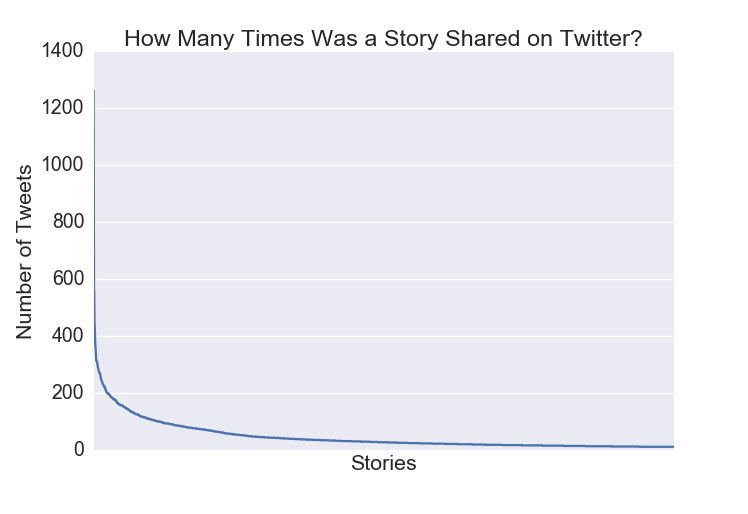
\includegraphics[width=\columnwidth]{story-share-dist}  
  \caption{Distribution of Story Shares
    \label{fig:story-share-dist}}
\end{figure} 


Story sharing behavior follows an approximate power law distribution. On average, stories are shared 46 times, however, the median (50th percentile) of shares is just 26. 


CNN, Politico, and Fox lead in publication popularity with the highest number of stories shared by tweets in our dataset-- likely due to the volume and close association to political content of the companies. Because our data pipeline detailed in the previous chapter looks for election-related news, outlets which focus on political news are more likely to show up in our results.


\begin{figure}[t!]  
\centering 
  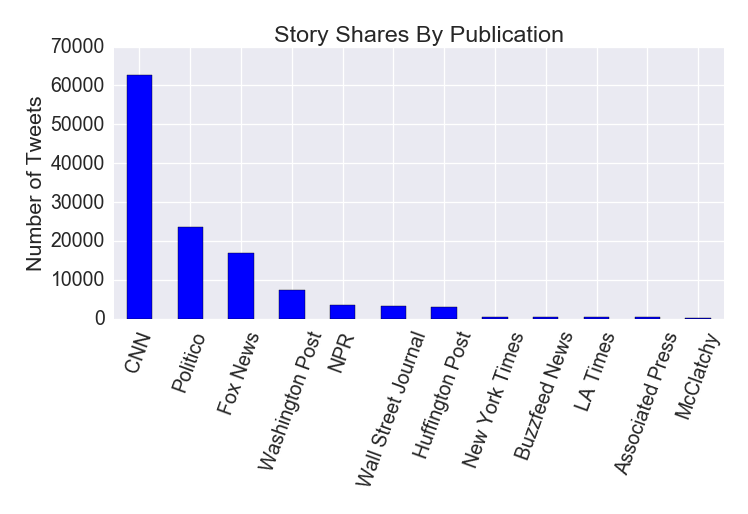
\includegraphics[width=\columnwidth]{all-stories-by-pub}  
  \caption{Number of story shares by publication
    \label{fig:tweets-by-pub}}
\end{figure} 


%\newpage %force table to get on the next page

Examining the top 10 most shared stories, it comes as no surprise that outsized personality Donald Trump is by far the most ``tweetable'' candidate, dominating the list with 7 out of 10 stories featuring his name in the title.

 
\begin{figure}[t!]  
\centering 
  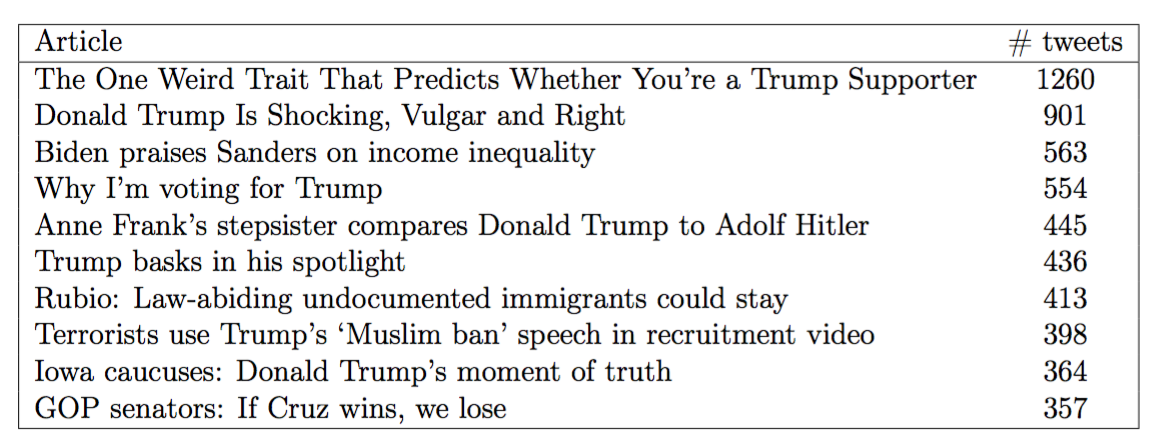
\includegraphics[width=\columnwidth]{top-10-stories}  
  \caption{Top 10 Most Shared Articles
    \label{fig:top-10-stories}}
\end{figure} 

% \begin{table} 
% \begin{tabular}{ |l c| } 
%     %s\toprule
%     \hline
%     Article &  \# tweets \\
%     \hline
%     %\midrule
%     The One Weird Trait That Predicts Whether You're a Trump Supporter &   1260 \\
%     Donald Trump Is Shocking, Vulgar and Right                         &    901 \\
%     Biden praises Sanders on income inequality                         &    563 \\
%     Why I'm voting for Trump                                           &    554 \\
%     Anne Frank's stepsister compares Donald Trump to Adolf Hitler      &    445 \\
%     Trump basks in his spotlight                                       &    436 \\
%     Rubio: Law-abiding undocumented immigrants could stay              &    413 \\
%     Terrorists use Trump's `Muslim ban' speech in recruitment video    &    398 \\
%     Iowa caucuses: Donald Trump's moment of truth                      &    364 \\
%     GOP senators: If Cruz wins, we lose                                &    357 \\
%     %\bottomrule
%     \hline
% \end{tabular}
% \caption{\label{tab:top-10}Top 10 Shared Stories}
% \end{table}

\begin{figure}[t!]  
\centering 
  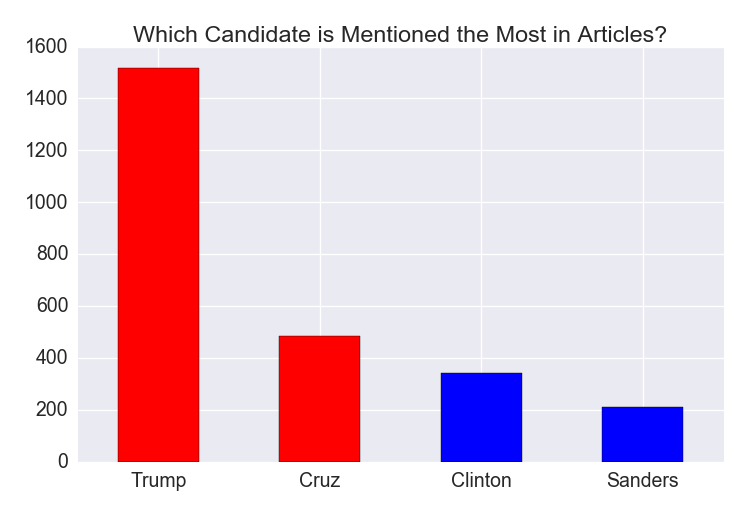
\includegraphics[width=\columnwidth]{candidate-mentions}  
  \caption{Most frequently mentioned candidate in stories
    \label{fig:tweets-by-pub}}
\end{figure} 


The extent to which he is prominent in articles is clear: by coding each story by the most frequently mentioned candidate mentioned in the body of the text, Trump has nearly three times as much coverage at nearly 60\% as the runner-ups, Ted Cruz and Hillary Clinton.

The large number of stories with Cruz as the most-mentioned candidate are likely due to his association to Trump as a Republican runner-up: 96\% of stories where Cruz is the most-mentioned candidate feature Trump as the second-most frequently occuring.
 

\section{Measuring Political and Emotional Engagement}

In the following sections, we discuss the tools and methods that we use to analyze our independent variables.

\subsection{Emotional Coding}
For the emotional coding of news articles, we use dictionaries from the Harvard General Inquirer, a lexicon that is popular for computerized content analysis \cite{stone1963computer}. In Berger and Milkman’s study of online virality, automated coding using the LIWC system showed results that were significantly positively correlated with the output of manual coding \cite{berger2012makes}. The Inquirer is a public-use alternative to the LIWC system. 

In particular, we use the \emph{Positiv} and \emph{Negativ} collections, a set of 1,915 well-established words signifying positive outlook (not including words for \emph{yes}) and 2,291 words signifying negative outlook (not including words for \emph{no}), respectively. Repeating the same metrics from \emph{What Makes Online Content Viral?}, we quantify for each document:

$$ emotionality = \frac{count(positiv \mid negativ)}{count(words)}$$
$$ positivity = \frac{count(positiv)}{count(words)} - \frac{count(negativ)}{count(words)}$$

as independent variables in our analysis.

 \subsection{Followership as a Proxy for Political Engagement}

In the following sections, we use Twitter followership as a proxy for measuring degrees of political engagement. 

Previous research in network analysis and attempts to predict latent political affiliations of users in the social network has shown that users on Twitter tend to show network homophily within political groups, and that ``like follows like''. In addition, followership of only Democratic or only Republican official accounts can be used as a reasonable estimator of party loyalty. Those accounts that follow only the officials of one party tend to demonstrate more closeness with other users in their political party than those who do not \cite{colleoni2014echo}.
            
Due to the highly individual nature of this election, where candidate loyalty does not necessarily imply goodwill towards the party, we look specifically at what candidates users follow. 

For general \emph{levels} of political engagement, we look at the number of political candidates a Twitter user follows as a proxy for how likely they are to share political news. 

In addition, for single-candidate Tweeters, we divide users by the candidate they follow. At the time of data collection completion (May 1, 2016), the top two candidates by delegate count in each party were Hillary Clinton (D), Bernie Sanders (D) and Donald Trump (R) and Ted Cruz (R), so we split users into these four groups. 

%We call each group \emph{X}-followers where \emph{X} is the candidate name, although these do not include every person on Twitter who follows \emph{X}.  

\subsubsection{Candidate Followership}

Our dataset contains 6,406 unique single-candidate Twitter users. Trump-only followers lead with about 31\%, followed closely by Clinton-only (29\%), then Sanders (25\%) and Cruz (14\%).


\begin{figure}[t!]  
\centering 
  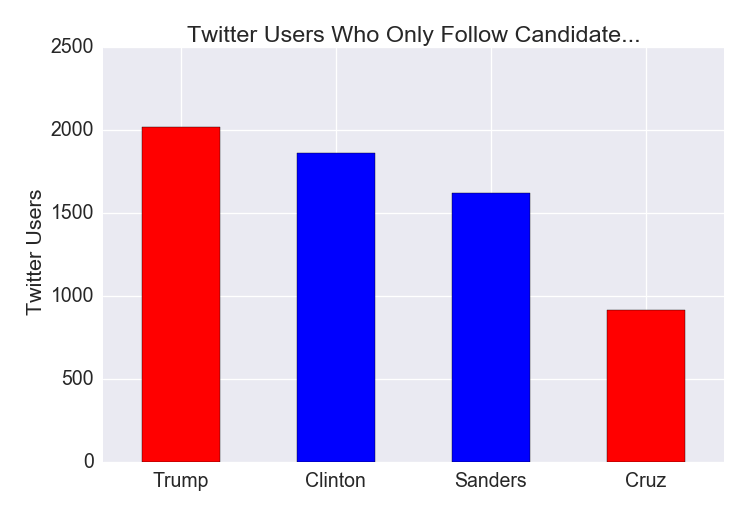
\includegraphics[width=\columnwidth]{users-by-candid}  
  \caption{Number of Tweets by Each Segment
    \label{fig:users-by-candid}}
\end{figure} 

 

Trump's free media advantage becomes clear when looking at the \emph{volume} of tweets each group of users tweet: 37\% of tweets sharing articles come from Trump-only followers versus 27\% for Clinton-only, 20\% for Sanders-only, and 14.6\% for Cruz.

\begin{figure}[t!]  
\centering 
  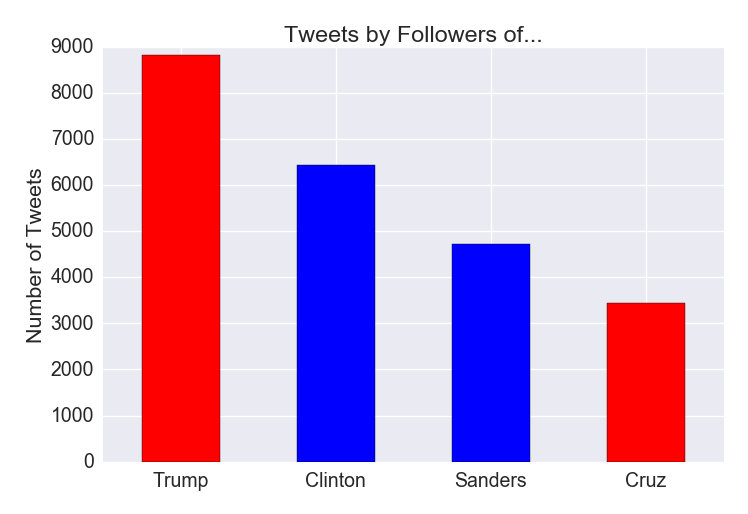
\includegraphics[width=\columnwidth]{tweets-by-candid}  
  \caption{Most frequently mentioned candidate in stories
    \label{fig:tweets-by-candid}}
\end{figure} 

We also observe the nature of the content being shared by each group. Again, across all four segments, Republican candidate Trump leads the top number of mentions in stories shared.

%% Most popular mentioned candidate by ea. camp
\begin{figure}[t!] 
\centering 
 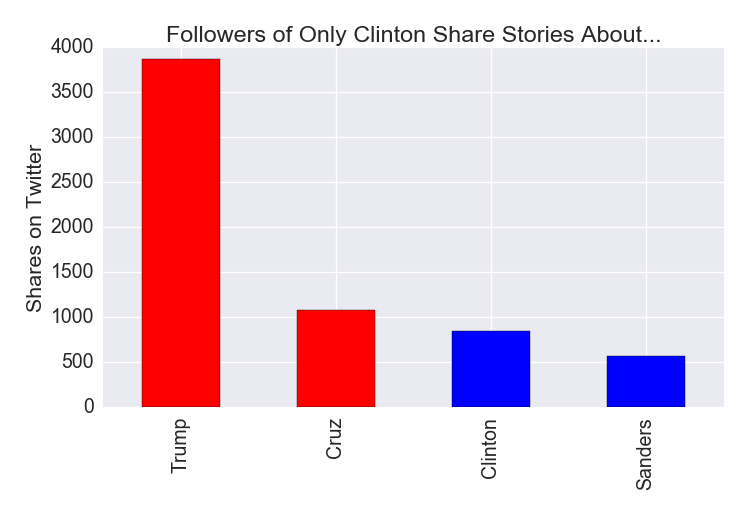
\includegraphics[width=0.49\columnwidth]{clinton-camp-shares}
 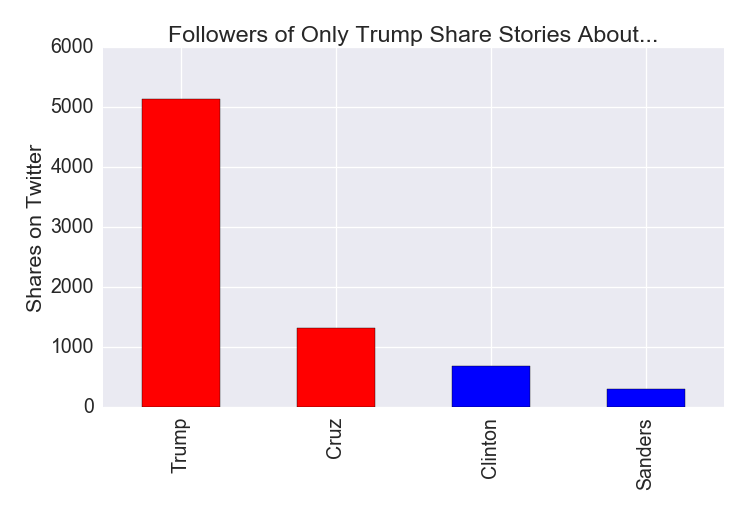
\includegraphics[width=0.49\columnwidth]{trump-camp-shares}  
 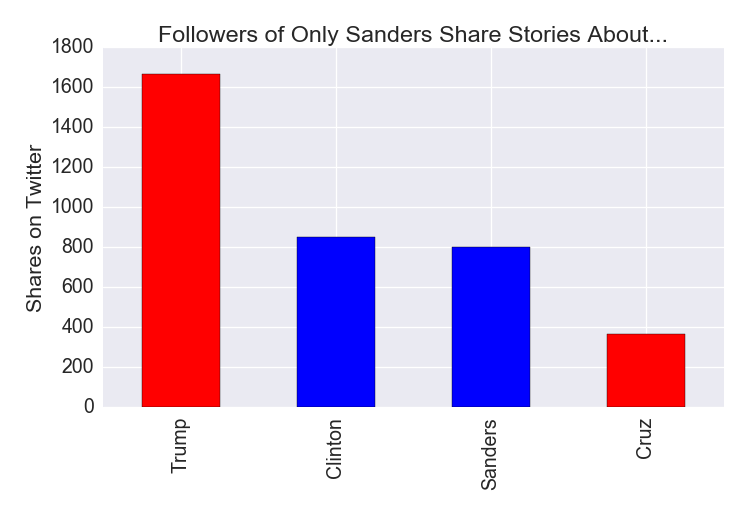
\includegraphics[width=0.49\columnwidth]{sanders-camp-shares}  
 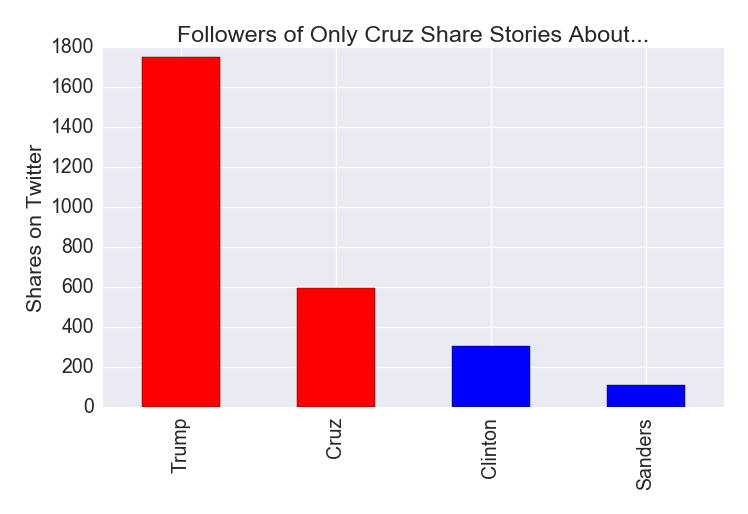
\includegraphics[width=0.49\columnwidth]{cruz-camp-shares}  
  %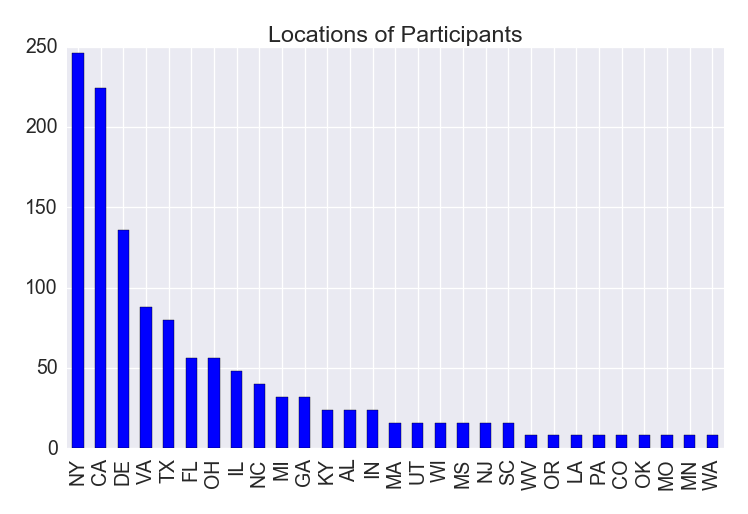
\includegraphics[width=0.32\columnwidth]{location_study2} 
  \caption{Tweet and User Counts by Followership
    \label{fig:users-tweets-by-candid}}
\end{figure}
 
\subsection{Political Engagement}

% Descriptives of candididate 0/1/3+:
% * Bar chart of \% by \# Following
% * Number of tweets by each camp
% * Most popular orgs by each camp
% * Most popular story by each camp
% * Most mentioned candid in each camp


\begin{figure}[t!]  
\centering 
  \includegraphics[width=1.0\columnwidth]{candid-ct}  
  \caption{Number of candidates followed
    \label{fig:candid-ct}}
\end{figure}

36\% of Twitter users in our dataset follow none of the four political candidates, followed by 31\% who follow one candidate, 20\% who follow two, and 13\% who follow three or more candidates. 


\begin{figure}[t!]  
\centering 
  \includegraphics[width=1.0\columnwidth]{tweets-by-candid-ct}  
  \caption{Ratio of Tweets to political candidates followed
    \label{fig:candid-ct}}
\end{figure}

We see a negative curvlinear relationship between the number of candidates followed (level of observed political engagement) and the ratio of political news tweets per user.


In the following analyses, we segment levels of political engagement into three groups for the sake of comparison:

\begin{itemize}
  \item \emph{the unaffiliated} (those who follow no presidential candidates, but do tweet about political news)
  \item \emph{the loyal} (those who follow one and only one presidential candidate, and tweet about political news)
  \item \emph{the political aficionados} (those who follow all 4 (or more) candidates, and tweet about political news).
\end{itemize}


\section{Analysis} 
For each of these three independent variables (story length, emotionality, positivity) we repeat analyses across three views of the data: first, the entire dataset; then, by political candidate followed amongst users who follow only one candidate; and finally, by the number of political candidates followed (degree of political engagement), to look for differences amongst different populations of political tweeters.


\subsection{Methodology}

Since our dependent variable, tweet volume, is a set of discrete counts that are positively truncated, we use negative binomial regression models for our analysis \cite{scott1997regression}. The distribution of tweet volume is not a normal distribution, and it is not recommended to perform a log transformation on count data to fit it to an OLS regression unless there is little dispersion in the data \cite{o2010not}. Poisson models are a subset of negative binomial models without the dispersion parameter. In our analyses, we see that the negative binomial model provides the best fit and that our data is overdispersed, as the dispersion parameter $\theta$ is greater than 1.   

In addition, we apply a log transformation on the independent variable of story length, as its distribution follows an approximate power law. Both emotionality and positivity are more normally distributed so we do not transform the data.
In each case, we compare our findings to those using linear and Poisson regression models, and are able to achieve the same significant results. 

%% IF NEC, YOU CAN INCLUDE THESE DISTRIBUTION CHARTS,
% %% BUT THAT MIGHT RAISE QUESTIONS ABOUT LEFT-SKEW OF POS., ETC.
% \begin{figure}[t!] 
% \centering 
%  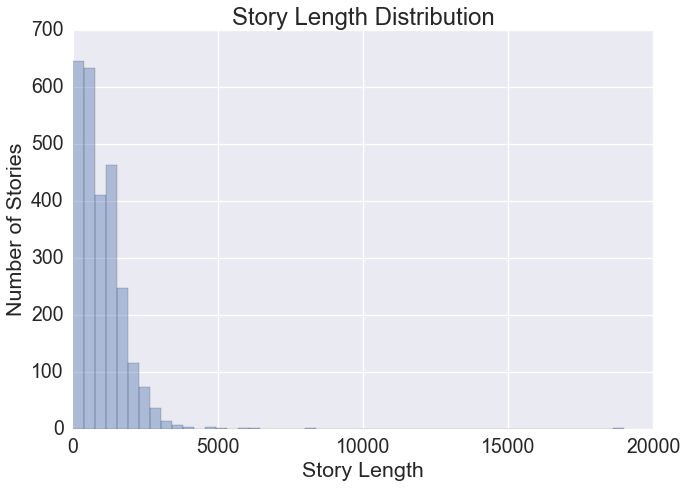
\includegraphics[width=1\columnwidth]{wc_dist}
%  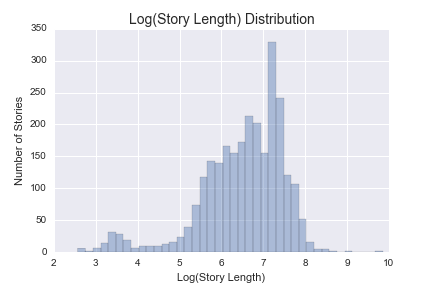
\includegraphics[width=1\columnwidth]{log_wc_dist}  
%  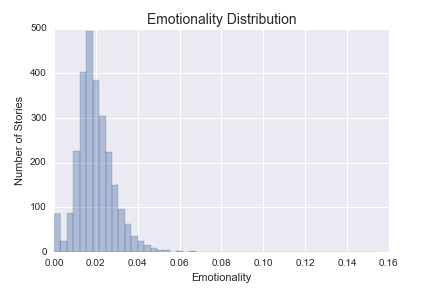
\includegraphics[width=1\columnwidth]{emot_dist}  
%  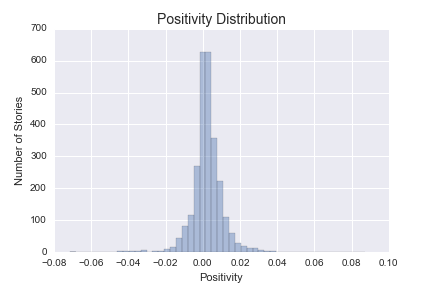
\includegraphics[width=1\columnwidth]{pos_dist}  
%   %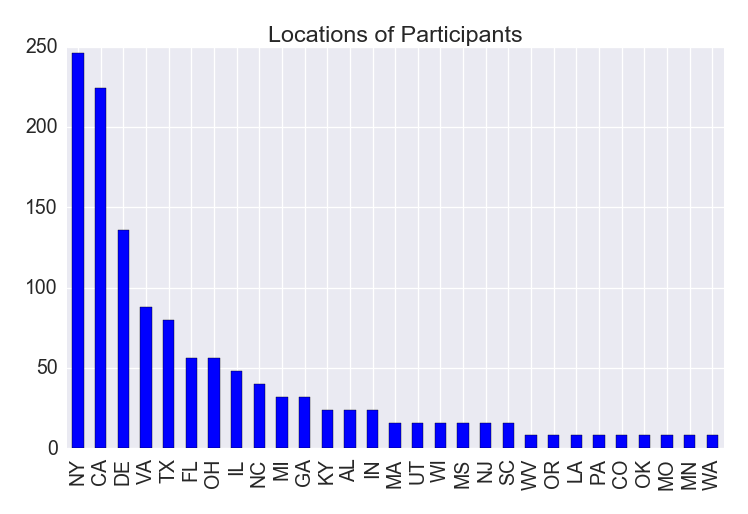
\includegraphics[width=0.32\textwidth]{location_study2} 
%   \caption{Tweet and User Counts by Followership
%     \label{fig:users-tweets-by-candid}}
% \end{figure}



\subsection{All Data}

% Table created by stargazer v.5.2 by Marek Hlavac, Harvard University. E-mail: hlavac at fas.harvard.edu
% Date and time: Thu, Dec 22, 2016 - 11:14:33
\begin{table}[!htbp] \centering 
  \caption{Story Popularity vs. Story Traits, All Tweets} 
  \label{} 
\begin{tabular}{@{\extracolsep{5pt}}lc} 
\\[-1.8ex]\hline 
\hline \\[-1.8ex] 
 & \multicolumn{1}{c}{\textit{Dependent variable:}} \\ 
\cline{2-2} 
\\[-1.8ex] & num\_tweets \\ 
\hline \\[-1.8ex] 
 log(wc) & $-$0.088$^{***}$ \\ 
  & (0.017) \\ 
  & \\ 
 emotionality & 6.279$^{***}$ \\ 
  & (1.770) \\ 
  & \\ 
 positivity & $-$5.978$^{***}$ \\ 
  & (2.013) \\ 
  & \\ 
 Constant & 4.296$^{***}$ \\ 
  & (0.117) \\ 
  & \\ 
\hline \\[-1.8ex] 
Observations & 2,650 \\ 
Log Likelihood & $-$12,761.660 \\ 
$\theta$ & 1.361$^{***}$  (0.035) \\ 
Akaike Inf. Crit. & 25,531.320 \\ 
\hline 
\hline \\[-1.8ex] 
\textit{Note:}  & \multicolumn{1}{r}{$^{*}$p$<$0.1; $^{**}$p$<$0.05; $^{***}$p$<$0.01} \\ 
\end{tabular} 
\end{table} 



\subsubsection{Story Length}
Overall, we find a consistently negative correlation of high significance between story length and Twitter volume ($\beta=-0.088$, $p<0.01$). 
This aligns with our hypothesis \textbf{H1:} that shorter stories are more likely to be shared, due to competing resources in the attention economy.

% \begin{figure}[t!]  
% \centering 
%   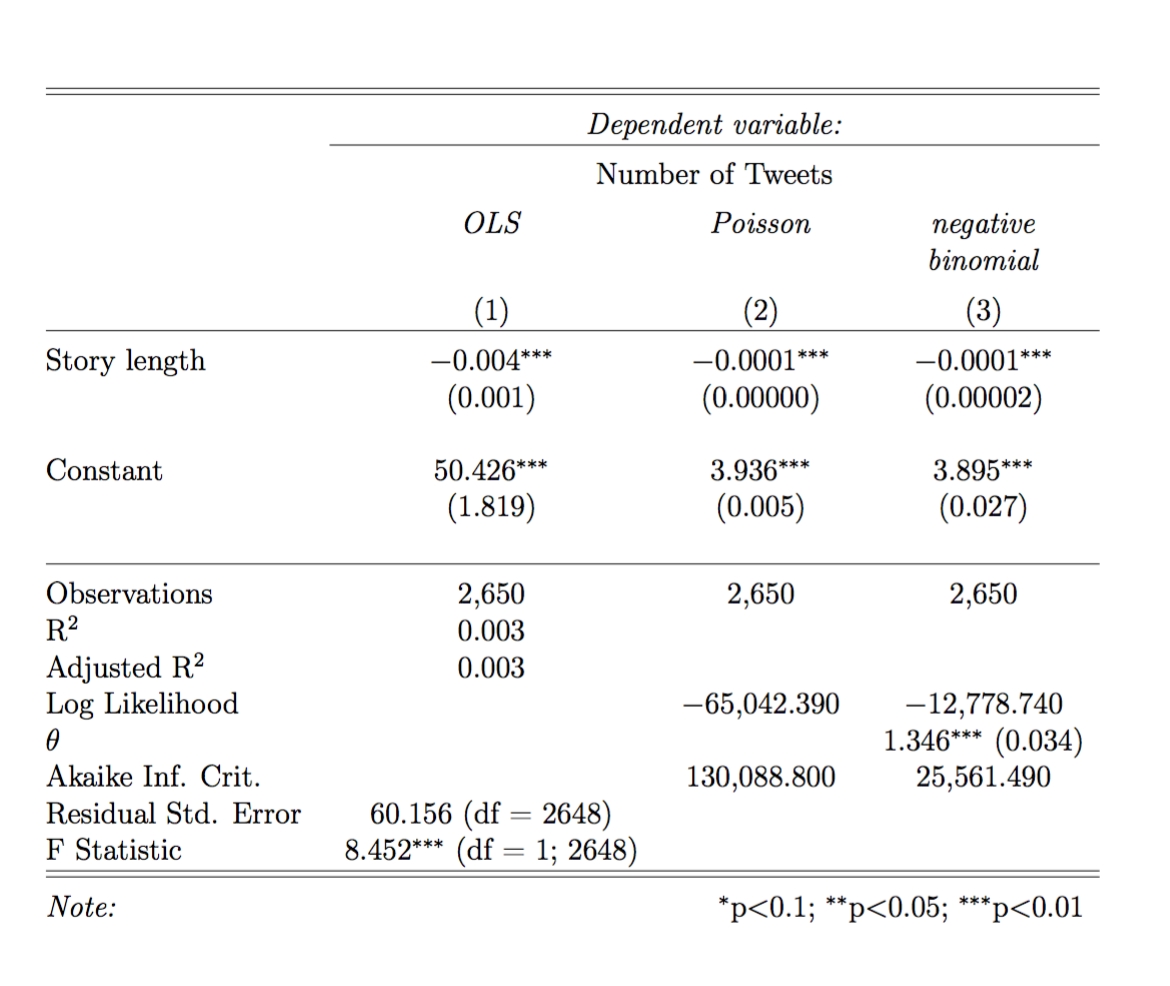
\includegraphics[width=1.0\columnwidth]{story-len-table}  
%   \caption{Tweet Volume vs. Story Length, All Tweets
%     \label{fig:story-len-table}}
% \end{figure}


% Table created by stargazer v.5.2 by Marek Hlavac, Harvard University. E-mail: hlavac at fas.harvard.edu
% Date and time: Sun, Jul 24, 2016 - 17:29:16
% \begin{table}[!t] \centering 
%   \caption{Tweet Volume vs. Story Length, All Data} 
%   \label{} 
%     \begin{tabular}{@{\extracolsep{5pt}}lccc} 
%     \\[-1.8ex]\hline 
%     \hline \\[-1.8ex] 
%      & \multicolumn{3}{c}{\textit{Dependent variable:}} \\ 
%     \cline{2-4} 
%     \\[-1.8ex] & \multicolumn{3}{c}{Number of Tweets} \\ 
%     \\[-1.8ex] & \textit{OLS} & \textit{Poisson} & \textit{negative} \\ 
%      & \textit{} & \textit{} & \textit{binomial} \\ 
%     \\[-1.8ex] & (1) & (2) & (3)\\ 
%     \hline \\[-1.8ex] 
%      Story length & $-$0.004$^{***}$ & $-$0.0001$^{***}$ & $-$0.0001$^{***}$ \\ 
%       & (0.001) & (0.00000) & (0.00002) \\ 
%       & & & \\ 
%      Constant & 50.426$^{***}$ & 3.936$^{***}$ & 3.895$^{***}$ \\ 
%       & (1.819) & (0.005) & (0.027) \\ 
%       & & & \\ 
%     \hline \\[-1.8ex] 
%     Observations & 2,650 & 2,650 & 2,650 \\ 
%     R$^{2}$ & 0.003 &  &  \\ 
%     Adjusted R$^{2}$ & 0.003 &  &  \\ 
%     Log Likelihood &  & $-$65,042.390 & $-$12,778.740 \\ 
%     $\theta$ &  &  & 1.346$^{***}$  (0.034) \\ 
%     Akaike Inf. Crit. &  & 130,088.800 & 25,561.490 \\ 
%     Residual Std. Error & 60.156 (df = 2648) &  &  \\ 
%     F Statistic & 8.452$^{***}$ (df = 1; 2648) &  &  \\ 
%     \hline 
%     \hline \\[-1.8ex] 
%     \textit{Note:}  & \multicolumn{3}{r}{$^{*}$p$<$0.1; $^{**}$p$<$0.05; $^{***}$p$<$0.01} \\ 
%     \end{tabular} 
% \end{table} 
% \newpage
 
\subsubsection{Emotionality}
Overall, we find a consistently positive correlation of high significance between emotionality and Twitter volume ($\beta=6.279$, $p<0.01$). 


% Table created by stargazer v.5.2 by Marek Hlavac, Harvard University. E-mail: hlavac at fas.harvard.edu
% Date and time: Sun, Jul 24, 2016 - 18:56:10
% \begin{table}[!t] \centering 
%   \caption{Tweet Volume vs. Emotionality, All Data} 
%   \label{} 
%     \begin{tabular}{@{\extracolsep{5pt}}lccc} 
%     \\[-1.8ex]\hline 
%     \hline \\[-1.8ex] 
%      & \multicolumn{3}{c}{\textit{Dependent variable:}} \\ 
%     \cline{2-4} 
%     \\[-1.8ex] & \multicolumn{3}{c}{Number of Tweets} \\ 
%     \\[-1.8ex] & \textit{OLS} & \textit{Poisson} & \textit{negative} \\ 
%      & \textit{} & \textit{} & \textit{binomial} \\ 
%     \\[-1.8ex] & (1) & (2) & (3)\\ 
%     \hline \\[-1.8ex] 
%      Emotionality & 305.229$^{**}$ & 6.111$^{***}$ & 6.019$^{***}$ \\ 
%       & (122.427) & (0.276) & (1.777) \\ 
%       & & & \\ 
%      Constant & 40.349$^{***}$ & 3.714$^{***}$ & 3.716$^{***}$ \\ 
%       & (2.685) & (0.006) & (0.039) \\ 
%       & & & \\ 
%     \hline \\[-1.8ex] 
%     Observations & 2,650 & 2,650 & 2,650 \\ 
%     R$^{2}$ & 0.002 &  &  \\ 
%     Adjusted R$^{2}$ & 0.002 &  &  \\ 
%     Log Likelihood &  & $-$65,180.470 & $-$12,779.510 \\ 
%     $\theta$ &  &  & 1.345$^{***}$  (0.034) \\ 
%     Akaike Inf. Crit. &  & 130,364.900 & 25,563.030 \\ 
%     Residual Std. Error & 60.181 (df = 2648) &  &  \\ 
%     F Statistic & 6.216$^{**}$ (df = 1; 2648) &  &  \\ 
%     \hline 
%     \hline \\[-1.8ex] 
%     \textit{Note:}  & \multicolumn{3}{r}{$^{*}$p$<$0.1; $^{**}$p$<$0.05; $^{***}$p$<$0.01} \\ 
%     \end{tabular} 
% \end{table} 

% \begin{figure}[t!]  
% \centering 
%   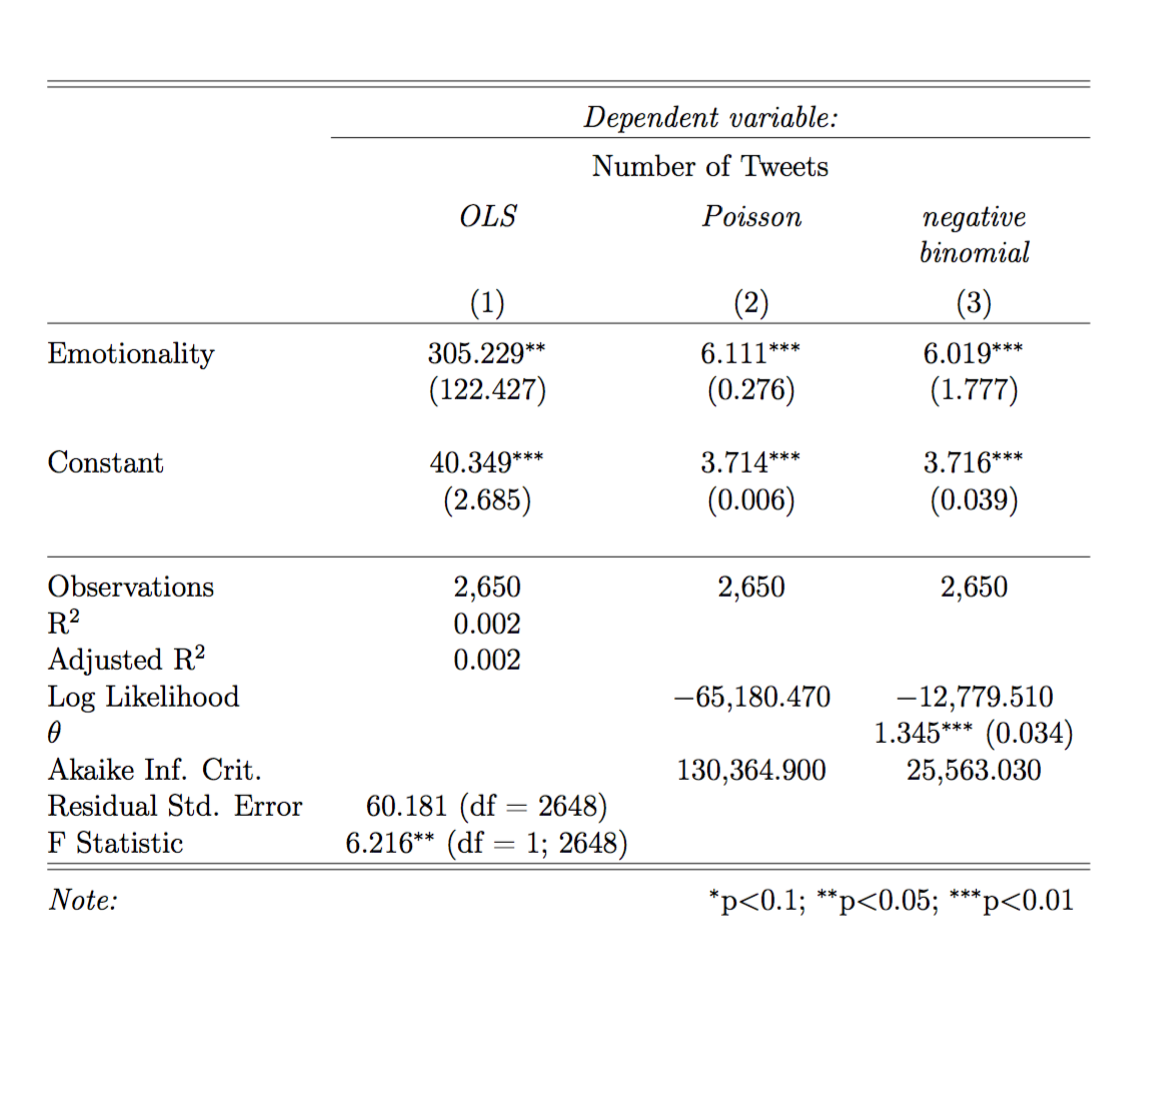
\includegraphics[width=1.0\columnwidth]{emot-table}  
%   \caption{Tweet Volume vs. Story Emotionality, All Tweets
%     \label{fig:emot-table}}
% \end{figure}


This confirms \textbf{H2:} that emotionality has a \emph{positive} correlation with Twitter shares, consistent for viral content in general \cite{berger2012makes}.

 
\subsubsection{Positivity}
Overall, we find a consistently negative correlation of high significance between positivity and Twitter volume ($\beta=−5.978$, $p<0.01$). 
 
% Table created by stargazer v.5.2 by Marek Hlavac, Harvard University. E-mail: hlavac at fas.harvard.edu
% % Date and time: Sun, Jul 24, 2016 - 18:58:37
% \begin{table}[!t] \centering 
%   \caption{Tweet Volume vs. Positivity, All Data} 
%   \label{} 
%     \begin{tabular}{@{\extracolsep{5pt}}lccc} 
%     \\[-1.8ex]\hline 
%     \hline \\[-1.8ex] 
%      & \multicolumn{3}{c}{\textit{Dependent variable:}} \\ 
%     \cline{2-4} 
%     \\[-1.8ex] & \multicolumn{3}{c}{Number of Tweets} \\ 
%     \\[-1.8ex] & \textit{OLS} & \textit{Poisson} & \textit{negative} \\ 
%      & \textit{} & \textit{} & \textit{binomial} \\ 
%     \\[-1.8ex] & (1) & (2) & (3)\\ 
%     \hline \\[-1.8ex] 
%      Positivity & $-$281.010$^{**}$ & $-$6.029$^{***}$ & $-$5.391$^{***}$ \\ 
%       & (139.546) & (0.338) & (2.029) \\ 
%       & & & \\ 
%      Constant & 47.078$^{***}$ & 3.851$^{***}$ & 3.849$^{***}$ \\ 
%       & (1.221) & (0.003) & (0.018) \\ 
%       & & & \\ 
%     \hline \\[-1.8ex] 
%     Observations & 2,650 & 2,650 & 2,650 \\ 
%     R$^{2}$ & 0.002 &  &  \\ 
%     Adjusted R$^{2}$ & 0.001 &  &  \\ 
%     Log Likelihood &  & $-$65,253.640 & $-$12,781.640 \\ 
%     $\theta$ &  &  & 1.343$^{***}$  (0.034) \\ 
%     Akaike Inf. Crit. &  & 130,511.300 & 25,567.270 \\ 
%     Residual Std. Error & 60.206 (df = 2648) &  &  \\ 
%     F Statistic & 4.055$^{**}$ (df = 1; 2648) &  &  \\ 
%     \hline 
%     \hline \\[-1.8ex] 
%     \textit{Note:}  & \multicolumn{3}{r}{$^{*}$p$<$0.1; $^{**}$p$<$0.05; $^{***}$p$<$0.01} \\ 
%     \end{tabular} 
% \end{table} 

% \begin{figure}[t!]  
% \centering 
%   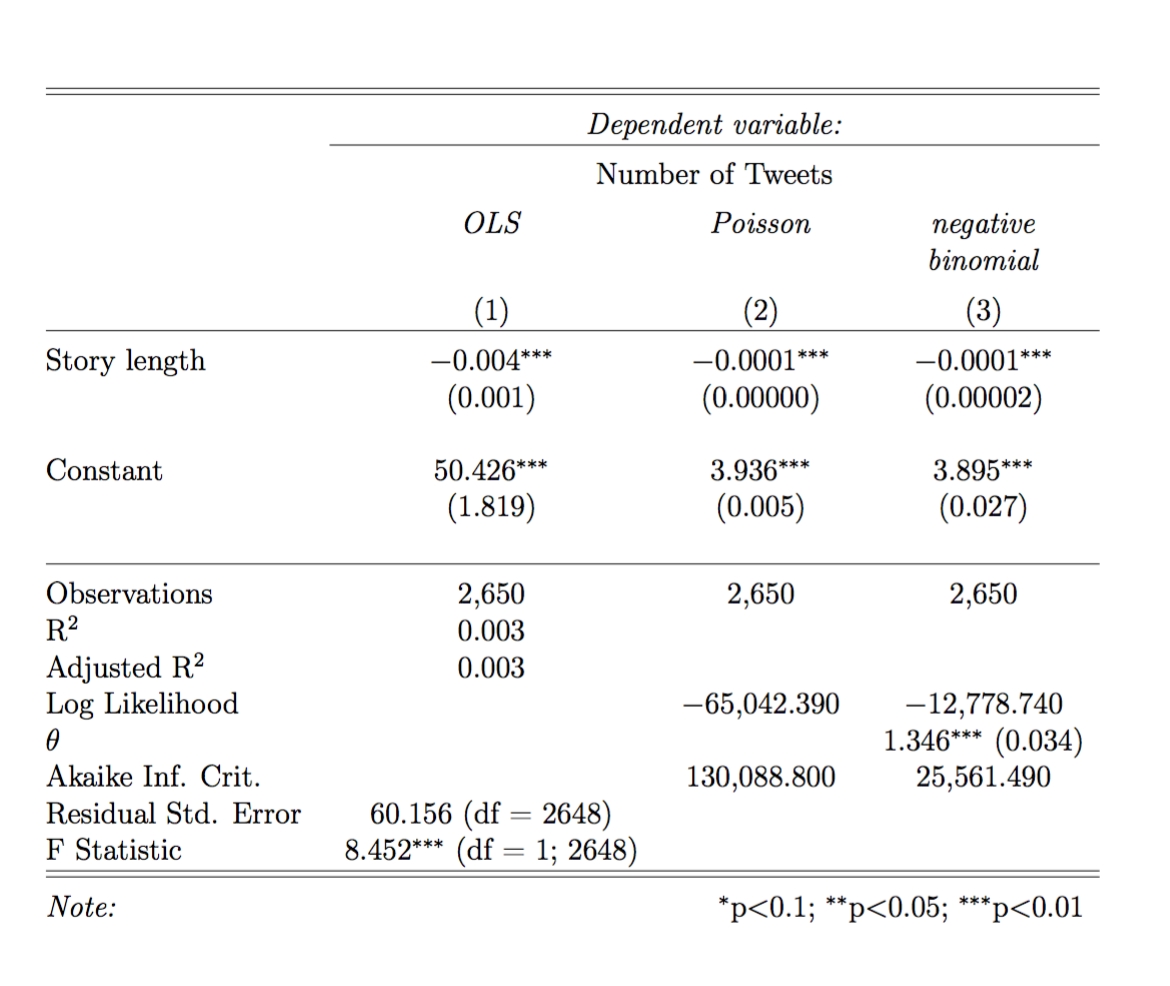
\includegraphics[width=1.0\columnwidth]{story-len-table}  
%   \caption{Tweet Volume vs. Positivity, All Tweets
%     \label{fig:story-len-table}}
% \end{figure}


This finding supports \textbf{H3:} Positivity has a \emph{negative} correlation with Twitter shares, due to the nature of political news and contrary to generalized findings \cite{berger2012makes}.

\subsection{By Degree of Political Engagement}

For the three levels of political engagement (the unaffiliated, single-candidate followers, and political aficionados) we repeat the same methods and variables in determining our correlations. Again, we test all three models (OLS, Poisson, and NB) for consistency and report the results of the negative binomial model.
 
 
Overall, we find that: 


\emph{The unaffiliated} show the same patterns as the general dataset with a negative correlation between story length and Twitter shares ($\beta=-0.283$, $p<0.01$), positive correlation between emotionality and Twitter shares ($\beta=10.718$, $p<0.01$), and a negative correlation between positivity and Twitter shares ($\beta=-4.968$, $p<0.05$).

\emph{The loyal}, on the other hand, show a slight positive correlation between story length and number of Twitter shares ($\beta=0.156$, $p<0.01$). For emotionality ($\beta=5.577$, $p<0.01$) and positivity ($\beta=-7.754$, $p<0.01$), the trends remain the same. We hypothesize that if following a single candidate can serve as a proxy for candidate loyalty, then perhaps the correlation signifies a willingness to read and share more complex content on behalf of the candidate and a deeper degree of political involvement.

We see the same effects for the \emph{political aficionados} group, again, a small but significant positive correlation between story length and number of tweets ($\beta=0.205$, $p<0.01$). For this group, we found no significant correlations between emotionality and Twitter popularity, although there was a significant negative correlation (as before) between positivity and tweets ($\beta=-6.043$, $p<0.05$). Again, this suggests a potential difference in levels of engagement with political news.
 

% % Table created by stargazer v.5.2 by Marek Hlavac, Harvard University. E-mail: hlavac at fas.harvard.edu
% % Date and time: Tue, Dec 27, 2016 - 12:45:31
% \begin{table}[!htbp] \centering 
%   \caption{Story Popularity vs. Story Traits, Single-Candidate Followers} 
%   \label{} 
% \begin{tabular}{@{\extracolsep{5pt}}lc} 
% \\[-1.8ex]\hline 
% \hline \\[-1.8ex] 
%  & \multicolumn{1}{c}{\textit{Dependent variable:}} \\ 
% \cline{2-2} 
% \\[-1.8ex] & num\_tweets \\ 
% \hline \\[-1.8ex] 
%  log(wc) & 0.156$^{***}$ \\ 
%   & (0.018) \\ 
%   & \\ 
%  emotionality & 5.577$^{***}$ \\ 
%   & (1.923) \\ 
%   & \\ 
%  positivity & $-$7.754$^{***}$ \\ 
%   & (2.200) \\ 
%   & \\ 
%  Constant & 1.125$^{***}$ \\ 
%   & (0.130) \\ 
%   & \\ 
% \hline \\[-1.8ex] 
% Observations & 2,581 \\ 
% Log Likelihood & $-$8,429.152 \\ 
% $\theta$ & 1.351$^{***}$  (0.040) \\ 
% Akaike Inf. Crit. & 16,866.300 \\ 
% \hline 
% \hline \\[-1.8ex] 
% \textit{Note:}  & \multicolumn{1}{r}{$^{*}$p$<$0.1; $^{**}$p$<$0.05; $^{***}$p$<$0.01} \\ 
% \end{tabular} 
% \end{table} 

% % Table created by stargazer v.5.2 by Marek Hlavac, Harvard University. E-mail: hlavac at fas.harvard.edu
% % Date and time: Tue, Dec 27, 2016 - 12:47:43
% \begin{table}[!htbp] \centering 
%   \caption{Story Popularity vs. Story Traits, Political Aficionados}
%   \label{} 
% \begin{tabular}{@{\extracolsep{5pt}}lc} 
% \\[-1.8ex]\hline 
% \hline \\[-1.8ex] 
%  & \multicolumn{1}{c}{\textit{Dependent variable:}} \\ 
% \cline{2-2} 
% \\[-1.8ex] & num\_tweets \\ 
% \hline \\[-1.8ex] 
%  log(wc) & 0.205$^{***}$ \\ 
%   & (0.022) \\ 
%   & \\ 
%  emotionality & $-$0.656 \\ 
%   & (2.330) \\ 
%   & \\ 
%  positivity & $-$6.043$^{**}$ \\ 
%   & (2.753) \\ 
%   & \\ 
%  Constant & $-$0.085 \\ 
%   & (0.160) \\ 
%   & \\ 
% \hline \\[-1.8ex] 
% Observations & 1,841 \\ 
% Log Likelihood & $-$4,224.546 \\ 
% $\theta$ & 2.370$^{***}$  (0.119) \\ 
% Akaike Inf. Crit. & 8,457.093 \\ 
% \hline 
% \hline \\[-1.8ex] 
% \textit{Note:}  & \multicolumn{1}{r}{$^{*}$p$<$0.1; $^{**}$p$<$0.05; $^{***}$p$<$0.01} \\ 
% \end{tabular} 
% \end{table} 

\subsection{By Candidate} 

We divide Twitter users into four segments: Trump-only, Clinton-only, Sanders-only, and Cruz-only followers and repeat the same regressions within each population. 

Overall, we were unable to find a significant difference in the direction of correlations in any of the three independent variables between these candidate groups and single-candidate followers (the loyal) at large. However, we did find differences in magnitudes of the coefficients; most notably a strong negative correlation between postivity and number of tweets for Trump-only followers, about two and a half times in magnitude ($\beta=-14.684$, $p<0.01$) of the rest of tweeters ($\beta=−5.978$, $p<0.01$). 

As discussed in the section above, all single-candidate followers that showed a significant correlation between story length and number of Twitter shares showed a slight positive correlation.

\section{Conclusion}

We find that, on the whole:
\begin{itemize}
    \item Shorter stories are more likely to be shared on Twitter (\textbf{H1})
    \item Stories high in emotional words, both negative and positive, are more likely to be shared on Twitter (\textbf{H2})
    \item Stories that are less positive are more likely to be shared on Twitter (\textbf{H3})
\end{itemize}

These results confirm our expectations of reader attention on the Internet, the emotional nature of content virality, and the negative connotation of political media. 

We were able to see small but significant differences in the number of political candidates a user followed and the length of the stories that were likely to be shared, suggesting differing degrees of political involvement. However, we were unable to find many significant differences between segments by specific political candidates that users followed. 

This suggests that either the characteristics of political news we examine (length, emotionality, positivity) are universal in their effects on motivating readers to share articles, or that our methods of dividing Twitter users do not reveal significant underlying differences between readers.


\section{Limitations \& Future Work}
Although we take a ``big data'' approach to our analysis, our dataset is by no means a complete mapping of \emph{all} political news sharing activity on Twitter. Our sources are limited to a small but diverse set of publications, which are by no means representative of all news outlets.

Furthermore, we match tweets with stories optimizing for efficiency and speed by using regular expressions, rather than completeness.

Potential paths of future research include:
\begin{itemize}
\item Expanding the set of publications tracked  
\item Replicating the analysis on a real-time basis
\item Using machine learning methods to match tweets with stories in a more intelligent way
\item Analyzing more nuanced emotive words in the text, in addition to positive and negative words
\item Looking at additional signals in the Twitter data, such as user characteristics of the sharer and network aspects of stories being shared
\item Segmenting Twitter users in different ways aside from candidates followed
 \end{itemize}

Still, this analysis provides a first view of article sharing on Twitter in a unique and eventful election year with large responses on social media.

 





\bibliography{nasty-brutish-short}
\bibliographystyle{aaai} 
 
\end{document}
